\documentclass[a4paper]{article}
\usepackage{graphicx}
\usepackage{amsmath, amsfonts, geometry, float, listings, enumerate, multicol}
\usepackage{multicol, float, color, colortbl}
\usepackage{tikz, titlesec, parskip, pgfplots, filecontents}
\usepackage{hyperref}
\usepackage{amsmath}
\usepackage{tikz, titlesec, parskip}
\usepackage{tikz,pgfplots}
\usepackage[americanvoltages,fulldiodes,siunitx]{circuitikz}
\usetikzlibrary{shapes,arrows}
\usepackage{enumitem}
\titleformat*{\subsubsection}{\LARGE\bfseries}

\titlespacing{\section}{0pt}{10pt}{0pt}
\titlespacing{\subsection}{0pt}{10pt}{0pt}
\titlespacing{\subsubsection}{0pt}{10pt}{0pt}



\usetikzlibrary{calc,patterns,through}
\newcommand{\arcangle}{%
	\mathord{<\mspace{-9mu}\mathrel{)}\mspace{2mu}}%
}

\renewcommand{\baselinestretch}{1.4}
 \geometry{
 a4paper,
 total={170mm,257mm},
 left=20mm,
 top=20mm,
 }
\usepackage{fancyhdr}
\usepackage{indentfirst}
\pagestyle{fancy}
\fancyhf{}
\rhead{\textbf{بهینه‌سازی در علوم داده}}
\lhead{\textbf{ میانترم }}
\cfoot{(\space \space \space \space \textbf{\thepage}  \space \space \space)}
\renewcommand{\headrulewidth}{1pt}
\renewcommand{\footrulewidth}{1pt}

 
\usepackage{xepersian}
\setlatintextfont{Times New Roman}
\settextfont{XB Niloofar}
\setdigitfont{XB Niloofar}
\DefaultMathsDigits

\makeatletter
\bidi@patchcmd{\@Abjad}{آ}{الف}
{\typeout{Succeeded in changing آ into الف}}
{\typeout{Failed in changing آ into الف}}
\makeatother
\PersianAlphs

\begin{document}
\begin{minipage}{0.6\textwidth}
\begin{bf}
\begin{center}
	\large
	به نام خدا\\
دکتر مجتبی تفاق - بهینه‌سازی در علوم داده \\
\Large
\vspace{0.4cm}
امیرحسین جوادی (97101489)
\end{center}
\end{bf}
\normalsize
\end{minipage} \hfill
\begin{minipage}{0.35\textwidth}
\begin{flushleft}
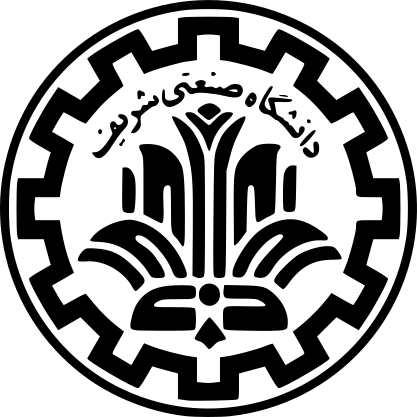
\includegraphics[width=0.5\textwidth]{logo.png}
\end{flushleft}
\begin{flushleft}
	دانشگاه صنعتی شریف\\
	دانشکده مهندسی برق\\
\end{flushleft}

\end{minipage}
\\
\rule[0.1\baselineskip]{\textwidth}{1pt}
\section{Q1}
\subsection{}
برای حل مسئله روبرو از نکته زیر استفاده کردم. 
\begin{equation*}
	x^{T}y = |x| |y| \cos(\angle(x,y)) \Rightarrow \cos(\angle(x,y)) = \frac{x^{T}y}{|x| |y|}
\end{equation*}
نکته‌ای که وجود دارد این است که زاویه‌ی بین دو بردار را میتوان با استفاده از ضرب داخلی به دست آورد. ایده‌ی روش بنده هم همین بود. من سعی کردم با داشتن ماتریس $ A $ و بردار $ x $ تخمینی از
 $ \cos(\alpha) $
 بزنم. برای این کار به تعداد 
 \lr{$ Train_size = 100000 $}
 داده برای یادگیری و 
 \lr{$ Test_size = 10000 $}
 برای تست کردن مدل نهایی به صورت تصادفی تولید کردم. هر داده یک آرایه‌ی $ 10 $ بعدی است که هر درایه‌ی آن یونیفرم در بازه‌ی
  $ [-1,1] $ 
  است. برای سهولت کار، من هم $ x $ و هم داده‌های یادگیری و تست را نرمالیزه کردم تا مخرج عبارت بالا برابر $ 1 $ باشد. برای هر داده‌ی تصادفی مثل $ z $، برچسب مربوطه را با کمک رابطه‌ی
   $ z^{T}Az $
   به دست آوردم. سپس لازم بود بیابم که کسینوس زاویه بین داده‌های با برچسب $ +1 $ و هم چنین با برچسب $ -1 $ در چه بازه‌ای بودند. برای این کار مدل خودم را همان بردار $ x $ فقط به صورت نرمالیزه شده در نظر گرفتم. سپس
    $ w = z^{T}x $
    را برای هر داده‌ حساب کردم. $ w $ مربوط به هر بچسب را از دیگری جدا کردم و ماکزیمم و مینیمم بازه‌ی کسینوس در هر دسته را به دست آوردم. از آن جایی که مسئله ما برای 
    $ z $ 
   و
     $ -z $
 یک برچسب اختصاص میدهد اندازه‌ی کسینوس باید مد نظر ما میبود. مقدار ترشهولد برای  اندازه‌ی کسینوس را برابر با مقدار زیر قرار دادیم.
\begin{equation*}
 	Threshold = \frac{\max_{1} + |\min_{1}| + \max_{-1} + |\min_{-1}|}{4}
\end{equation*}
   که اعداد زیر مینیمم و ماکزیمم دسته‌ی مورد نظر را نشان میدهند. برای سنجش کار خود دقت را روی داده‌ی آموزش و تست به دست آوردیم که به صورت زیر شد.
\begin{center}
	   \begin{latin}
   	The precision of my classifier on training data is 97.857\%
   	\\
   	The precision of my classifier on test data is 97.74\%
   \end{latin}
\end{center}
\subsection{}
\newpage
\section{Q2}
\subsection{}
ماتریس خالی به سایز 
$ [6000,5000] $
ساختم و خطوط 
$ v_{1}[k] $
و
$ v_{2}[k] $
را در شکل کشیدم. سعی کردم کمی قطور تر خطوط رو رسم کنم تا به چشم بیایند. تصویر به شکل زیر در آمد. 
\begin{figure}[H]
	\centering
	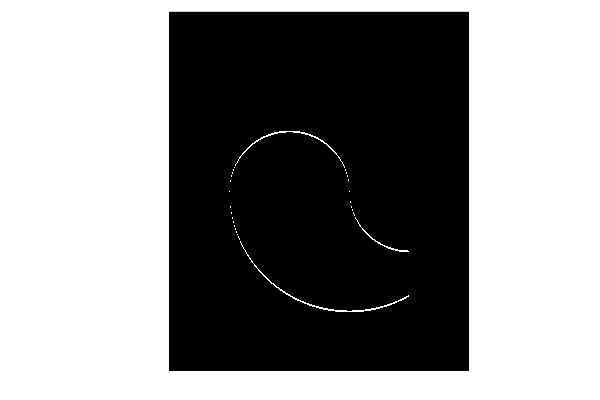
\includegraphics[width=0.75 \linewidth]{heatmap}
	\caption{
		\lr{Heatmap of Image}
	}
\end{figure}
رویه کار به این صورت خواهد بود که دو بردار 
$ v_{1}[k] $
و
$ v_{2}[k] $
را در بازه‌ی 
$ [1000:4000] $
داریم. سعی میکنیم توابعی در این بازه پیدا کنیم که تا جای ممکن به هر کدام از بردارها نزدیک باشند. سپس از این توابع برای تخمین عکس در قسمت مجهول استفاده می‌کنیم. 
کلیت شکل به توابع سینوسی و کسینوسی شبیه بود. برای همین از این توابع برای 
\lr{feature engineering}
استفاده کردم.
\subsection{}
همان طور که گفتیم کلیت شکل بسیار به توابع سینوسی و کسینوسی شبیه است. برای همین یک دوره برای
$ v_{1}[k] $
که برابر است با 
$ T_{v_{1}} = 4000 $
تخمین زدم. همچنین برای 
$ v_{2}[k] $
هم یک دوره برابر با
$ T_{v_{1}} = 8000 $
تخمین زدم. سپس توابع 
\lr{feature engineering}
را به شکل زیر تعریف کردم. 
\begin{equation*}
	\begin{cases}
		f_{0} = 1 \\
		f_{i} = \sin(\frac{2 \pi t}{T k^{i-1}}) & \text{for} $ i = 1:9 $ \\
		f_{i} = \sin(\frac{2 \pi k^{i-9} t}{T}) & \text{for} $ i = 10:17 $ \\
		f_{i} = \cos(\frac{2 \pi t}{T k^{i-18}}) & \text{for} $ i = 18:26 $ \\
		f_{i} = \cos(\frac{2 \pi k^{i-26} t}{T}) & \text{for} $ i = 27:34 $ \\
	\end{cases}
\end{equation*}
برای جلوگیری از 
\lr{overfitting}
یک ترم رگولاریزیشن قرار دادم. کلیت این ترم به این صورت است که سعی کردم برای $ f_{0} $ که متناظر با مقدار ثابت بود مقداری قرار ندهم و برای توابع سینوسی و کسونوسی با افزایش فرکانس وزن بیشتری برای رگولاریزه کردن قرار دادم. سپس دو مدل برای 
$ v_{1}[k] $
و
$ v_{2}[k] $
به دست آوردم که به شکل زیر شد. 
\begin{figure}[H]
	\centering
	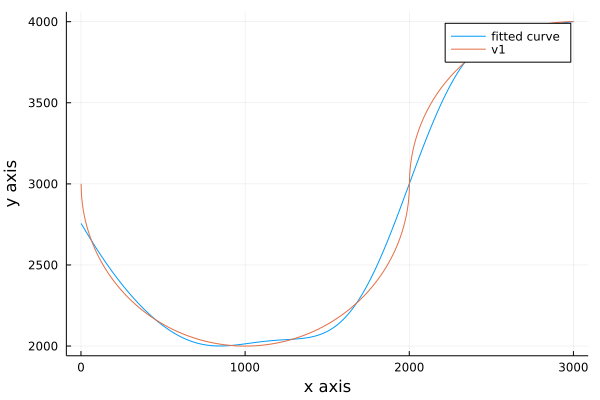
\includegraphics[width=0.75 \linewidth]{V1_fit}
	\caption{
		\lr{V1 points and fitted curve}
	}
\end{figure}
\begin{figure}[H]
	\centering
	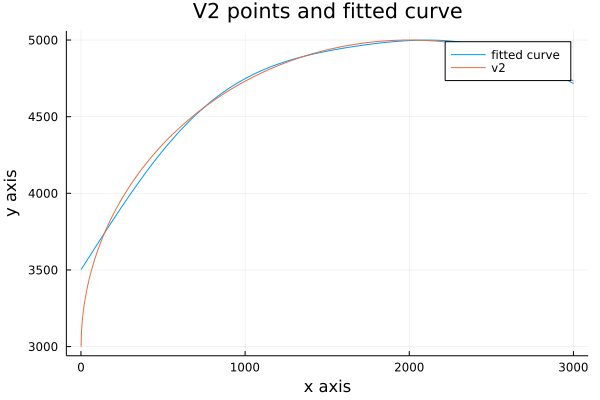
\includegraphics[width=0.75 \linewidth]{V2_fit}
	\caption{
		\lr{V2 points and fitted curve}
	}
\end{figure}
خطای 
\lr{Rms}
برای این دو مدل به شکل زیر شد: 
\begin{center}
	\begin{latin}
	Root mean squared loss of fitted curve on v1 is 60.73365435142669
	\\
	Root mean squared loss of fitted curve on v2 is 41.78805497174969
\end{latin}
\end{center}
سپس تکه‌ی نامشخص عکس را با استفاده از این دو معادله کشیدم و در کنار تکه دیگر گذاشتم که نتایج زیر به دست آمد.
\begin{figure}[H]
	\centering
	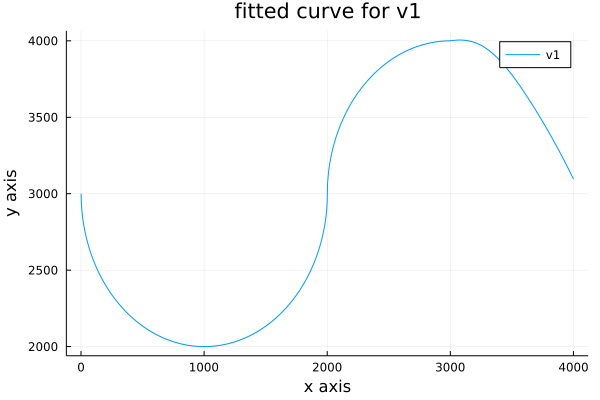
\includegraphics[width=0.75 \linewidth]{V1_curve}
	\caption{
		\lr{fitted curve for v1}
	}
\end{figure}
\begin{figure}[H]
	\centering
	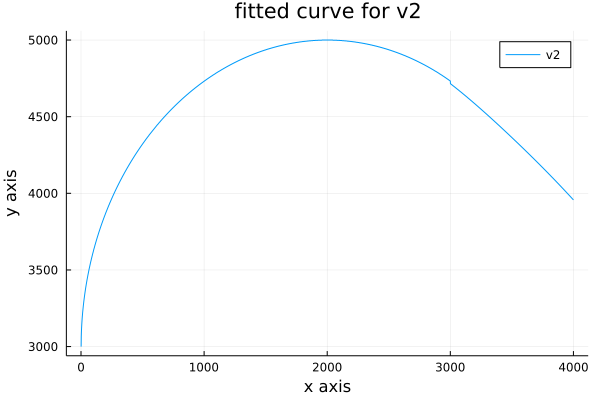
\includegraphics[width=0.75 \linewidth]{V2_curve}
	\caption{
		\lr{fitted curve for v2}
	}
\end{figure}
عکس نهایی هم به شکل زیر شد.
\begin{figure}[H]
	\centering
	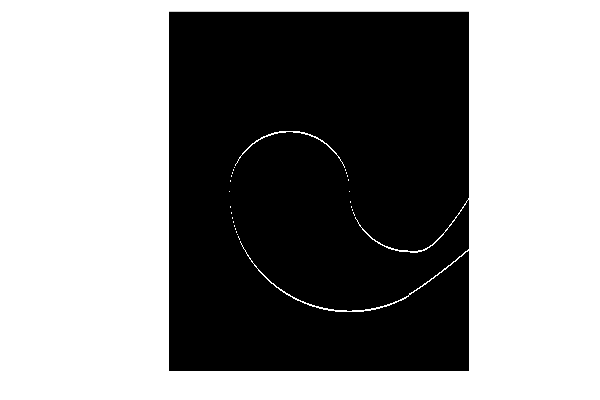
\includegraphics[width=0.75 \linewidth]{Reconstructed_Image}
	\caption{
		\lr{Reconstructed Image}
	}
\end{figure}
\subsection{}
از آن جایی که فقط داده‌های تصویر 
$ B $
‌را داریم شاید تنها خطایی که میتوان تعریف کرد پیدا کردن اختلاف این مدل و شکل واقعی در همین بازه است. من سعی کردم ملاک‌های دیگری هم لحاظ کنم مثل جلوگیری از وزن زیاد در فرکانس‌های بالا یا شبیه شدن 
\lr{curve}
نهایی به شکل سینوسی. 
\subsection{}
\begin{figure}[H]
	\centering
	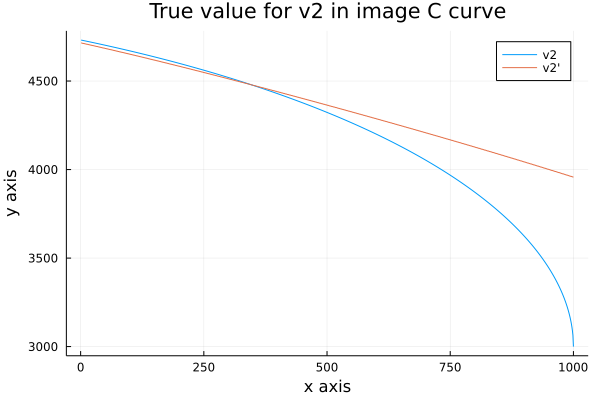
\includegraphics[width=0.75 \linewidth]{V2_curve_in_C}
	\caption{
		\lr{True value for v2 in image C curve}
	}
\end{figure}
\begin{center}
	\begin{latin}
		Root mean squared loss of fitted curve on v2 in image C is 11.732622212519468
	\end{latin}
\end{center}
\newpage
\section{Q3}
\subsection{}
جواب این مسئله باید چند ویژگی داشته باشد. اول این که جریان هر یال باید نامنفی باشد تا در جهت یال جریان داشته باشیم. دوم این که جریان هر یال از $ 1 $ بیشتر نخواهد بود. سوم این که جریان‌های ورودی هر گره برابر با جریان‌های خروجی هر گره باشد (به جز گره‌های ورودی و خروجی). بعد از نام گذاری یال‌ها، برای هر گره یک بردار به طول $ m $ در نظر میگیریم و به صورت زیر تعریف میکنیم. در ادامه فرض میکنیم که به گره $ s $  شماره‌ی $ 1 $ و به گره $ t $ شماره‌ی $ n $ تخصیص میدهیم
\begin{equation*}
	\text{\lr{For node $ i \Rightarrow $ }} a_{i}^{T}: \begin{cases}
		a_{ij} = 1  & \text{\lr{if edge $ j $ is goint to node $ i $}} \\
		a_{ij} = -1 & \text{\lr{if edge $ j $ is leaving node $ i $}} \\
		a_{ij} = 0 & \text{\lr{Otherwise}} \\
	\end{cases} 
\end{equation*}
پس قیود مسئله ما به شکل زیر است.
\begin{gather*}
	\begin{bmatrix}
		0 \\
		0 \\
		0 \\
		\vdots \\
		0 \\
		0 
	\end{bmatrix}
	\preceq
	\begin{bmatrix}
		1 & 0 & 0 & \dots & 0 & 0 \\
		0 & 1 & 0 & \dots & 0 & 0 \\
		0 & 0 & 1 & \dots & 0 & 0 \\
		\vdots & \vdots & \vdots & \vdots & \vdots & \vdots \\
		0 & 0 & 0 & \dots & 1 & 0 \\
		0 & 0 & 0 & \dots & 0 & 1 
	\end{bmatrix}
	\begin{bmatrix}
		f_{1} \\
		f_{2} \\
		f_{3} \\
		\vdots \\
		f_{m-1} \\
		f_{m} 
	\end{bmatrix}
	\preceq
	\begin{bmatrix}
		1 \\
		1 \\
		1 \\
		\vdots \\
		1 \\
		1 
	\end{bmatrix}
	\\
	\begin{bmatrix}
		a_{21} & a_{22} & a_{23} & \dots & a_{2(m-1)} & a_{2m} \\
		a_{31} & a_{32} & a_{33} & \dots & a_{3(m-1)} & a_{3m} \\
		a_{41} & a_{42} & a_{43} & \dots & a_{4(m-1)} & a_{4m} \\
		\vdots & \vdots & \vdots & \vdots & \vdots & \vdots \\
		a_{(n-2)1} & a_{(n-2)2} & a_{(n-2)3} & \dots & a_{(n-2)(m-1)} & a_{(n-2)m} \\
		a_{(n-1)1} & a_{(n-1)2} & a_{(n-1)3} & \dots & a_{(n-1)(m-1)} & a_{(n-1)m} \\
	\end{bmatrix}
	\begin{bmatrix}
		f_{1} \\
		f_{2} \\
		f_{3} \\
		\vdots \\
		f_{m-1} \\
		f_{m} 
	\end{bmatrix}
	=
	\begin{bmatrix}
		0 \\
		0 \\
		0 \\
		\vdots \\
		0 \\
		0 
	\end{bmatrix}
\end{gather*}
توجه شود که تعداد سطر‌های شرط دوم برابر $ n-2 $ است و برای گره‌های $ s $ و $ t $ این شرط را نداریم.
همچنین مقداری که می‌خواهیم ماکزیمم کنیم (شار خروجی از گره‌ی $ s $) برابر است با  اندازه‌ی مقدار زیر (مقدار زیر شار خارج شده از $ s $ است که مقدار منفی دارد. پس اندازه‌اش برایمان مهم است.)   
\begin{equation*}
	\begin{bmatrix}
		a_{11} & a_{12} & a_{13} & \dots & a_{1(m-1)} & a_{1m} 
	\end{bmatrix}
	\begin{bmatrix}
		f_{1} \\
		f_{2} \\
		f_{3} \\
		\vdots \\
		f_{m-1} \\
		f_{m} 
	\end{bmatrix} = a_{1}^{T} f
\end{equation*}
پس برای ماتریس $ A $ میتوانیم آرایه‌ی $ a_{1}^{T} $ را معرفی کنیم. پس حل مسئله‌ی ماکزیمم شار برابر شد با ماکزیمم سازی مقدار 
$ a_{1}^{T} f $ 
بر روی قیود $ f $.
\subsection{}
شار ماکزیمم برابر است با تعداد یالهای خارج شونده از $ s $. از آن جایی که ظرفیت هر یال حداکثر یک است شار خروجی از  $ s $ نمیتواند از این بیشتر شود. 
\begin{equation*}
	b = | \sum_{i=1}^{n} a_{1i} |
\end{equation*}
\subsection{}
طبق فورمول بندی که من کردم $ A $ یک آرایه است که خطی است. شرطی برابری روی $ f $   ستون هایش مستقل خطی نیست چون مثلا
 $ f = [1 1 \dots 1] $
 در 
 \lr{null space }
 آن است.
\subsection{}
برای حل این مسئله به این شیوه عمل میکنیم که شرط g مان دقیقا همان شرط برابر است و شرط h برابر است با
\begin{gather*}
	h(f) = || a_{1}^{T}f - a_{1}^{T} 1 || 
\end{gather*}
\subsection{}
\subsection{}
\newpage
\section{Q4}
\subsection{}
برای این سوال از روش 
\lr{K means}
استفاده کردم. این روش یک روش برای 
\lr{clustring}
است. این روش در اسلایدهای 
\lr{vlms} 
در فصل $ 4 $ ارائه شده است. این روش بر پایه یک الگوریتم 
\lr{iterative}
است که در آن در هر مرحله 
\lr{centroids}
یا مراکز دسته‌ها و سپس 
\lr{partition}
گروه هر داده به روز رسانی میشود. اول از همه داده‌ها را کشیدم. شکلی مانند شکل زیر داشت. 
\begin{figure}[H]
	\centering
	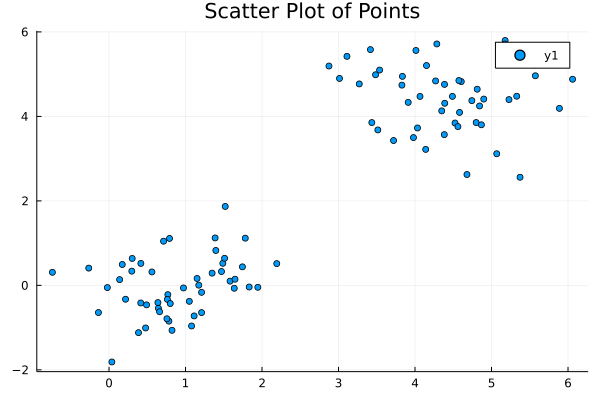
\includegraphics[width=0.75 \linewidth]{DataScattet}
	\caption{
		\lr{Scatter Plot of Points}
	}
\end{figure}

اول از همه دو مرکز رندوم تشکیل دادم. این کار در تابع 
\lr{Rand\_Z}
انجام شده است و به این صورت است که مینیمم و ماکزیمم طول و عرض داده‌ها را به دست آوردم. سپس یک عدد رندوم یونیفرم در بازه‌ی 
$ [0,1] $
تولید کردم و آن را به بازه‌ی متناظر در طول و عرض انتقال دادم. سپس 
\lr{criterion}
 را به صورتی در نظر گرفتم که الگوریتم حداکثر به اندازه‌ی 
 \lr{$ max\_iteration = 10000 $}
 بار الگوریتم اجرا شود. همچنین اگر در مرحله‌ای مراکزمان  هر دو از جایشنان تکان نخوردند الگوریتم 
 \lr{converge}
 میکند. در هر مرحله از الگوریتم اول هر داده به مرکزی که به آن نزدیک‌تر است متعلق میگیرد. این کار در تابع
 \lr{Partition}
 انجام شده است. سپس مرکز هر دسته در تابع 
 \lr{Centroids}
 به میانگین داده‌های در آن دسته به روز رسانی میشود. نتیجه نهایی به شکل زیر شد. 
\begin{figure}[H]
	\centering
	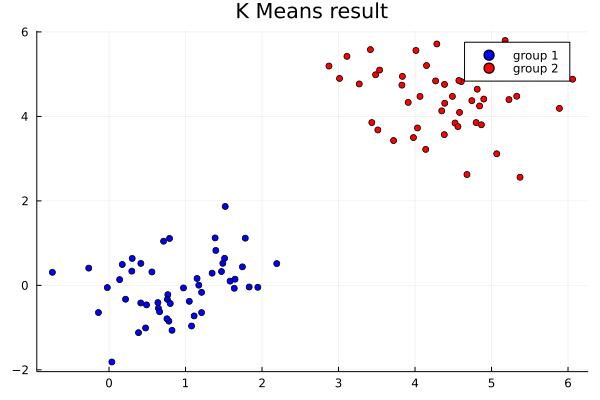
\includegraphics[width=0.75 \linewidth]{res1}
	\caption{
		\lr{Scatter Plot of Points}
	}
\end{figure}
\subsection{} 
فاصله بین نقطه‌ی
 $ t = [x_{0} , y_{0}]$
  و خط
 $ L : \{(x,y) | ax+by+c=0 \}  $
 برابر است با 
 \begin{equation*}
 	d = \frac{|ax_{0}+b y_{0}+c|}{\sqrt{a^{2} + b^{2}}}
 \end{equation*}
فاصله ی مرکز با این صفحه پس برابر است با 
\begin{equation*}
	d_{org} = \frac{|c|}{\sqrt{a^{2} + b^{2}}}
\end{equation*}
اگر دو دسته با استفاده از دو صفحه‌ی 
$ L_{1} : \{(x,y) | ax+by+c=1 \}  $
و 
$ L_{2} : \{(x,y) | ax+by+c=-1 \}  $
هم جدا بمانند دلخواه ما این است که تا جایی که میشود فاصله‌ی این دوصفه را از هم زیاد کنیم تا خطی با مارجین زیاد داشته باشیم. 
فاصله بین خطوط $ L_{1} $ و  $ L_{2} $ با هم برابر است با 
\begin{equation*}
	d_{12} = |\frac{|c-1|}{\sqrt{a^{2} + b^{2}}} - \frac{|c+1|}{\sqrt{a^{2} + b^{2}}}| = \frac{2}{\sqrt{a^{2} + b^{2}}}
\end{equation*}
پس ما به دنبال ضرایبی هستیم که 
\begin{gather*}
	\text{\lr{maximize : }} \frac{2}{\sqrt{a^{2} + b^{2}}}
	\\
	\text{\lr{Subject to : }} \begin{cases}
		ax + by + c \geq 1  & z = 1 \\
		ax + by + c \leq -1  & z = -1
	\end{cases}
\end{gather*}
در این رابطه $ z $ برابر دسته‌ی داده‌ها است. این برابر است با 
\begin{gather*}
	\text{\lr{minimize : }} a^{2} + b^{2}
	\\
	\text{\lr{Subject to : }} z(ax + by + c) \geq 1 \Rightarrow a (zx) + b (zy) + c(z) \geq 1
\end{gather*}
سعی میکنیم مسئله را به همین شیوه حل کنیم. پس 
\begin{gather*}
	f = a^{2} + b^{2} \qquad g = a (zx) + b (zy) + c(z) = 1
\end{gather*}
\newpage
\section{Q5}
\subsection{}
مقدار کمینه‌ی $ p $ برابر است با 
$ p = dim(null(A)) $
است. مجموعه‌ی ما ورژن شیفت یافته از 
\lr{hyperplane}
زیر است. 
\begin{equation*}
	C =  \{x | Ax = 0 \}
\end{equation*}
از آن جایی که 
$ By $ 
برابر است با اسپن ستون‌های $ B $ پس نتیجه میگیریم که ماتریس $ B $ باید ماتریسی باشد که اسپن ستون‌هایش بعد 
\lr{null space}
ماتریس $ A $ شود. 
برای پیدا کردن ستون‌های $ B $ باید بردارهای عمود بر سطرهای $ A $ را بیابیم. برای این کار میتوانیم از الگوریتم گرام اشمیت استفاده کنیم. بعد از استفاده از این روش به تعداد بعد 
\lr{null space}
بردار $ m $ بعدی خواهیم داشت و هر کدام را در یک ستون در ماتریس $ B $ قرار میدهیم. حال فقط مانده که $ b $ را به دست بیاوریم. برای این کار قرار میدهیم:
\begin{equation*}
	A =  \{x | Ax = a \} = \{By+b | A(By+b) = a , y \in R^{m}\} = \{By+b | Ab = a, y \in R^{m}\}
\end{equation*}
نامساوی آخر به این دلیل بود که $ By $ در 
\lr{null space}
ماتریس  $ A $ است. 
پس $ A $ برابر میشود با 
$ A^{\dagger}a $
\subsection{}
این جا باز هم به همان شکل عمل میکنیم. ستون‌های $ B $ پایه‌های 
\lr{null space}
ماتریس $ A $ است. پس با الگوریتم گرام اشمیت  میتوانیم بردارهای عمود بر آن ها را پیدا کنیم. سپس این بردارها را در سطر های یک ماتریس میگذاریم و به نتیجه نهایی میرسیم. برای پیدا کردن $ a $ به شکل زیر عمل کنیم. 
\begin{equation*}
	a = Ax = A(By+b) = Ab
\end{equation*}
\subsection{}
الگوریتم 
\lr{Gram Schmidt }
را در جولیا پیاده سازی کردم. فایل پیاده سازی شده موجود است. ماتریس نهایی به شکل زیر شد. 
\begin{equation*}
	A = \begin{bmatrix}
		 0.598902  &   0.515485  & -0.492619 &  0.0197789 & -0.364043 \\
		-1.46716e-15 & 0.0756714 & -0.497317 & -0.416091  &  0.757507
	\end{bmatrix}
	\quad
	a = \begin{bmatrix}
		6.959631187105747 \\
		7.064638955085694
	\end{bmatrix}
\end{equation*}
\subsection{}
این یک مسئله مینیمم سازی مقید است. ما به دنبال $ x $ و $ y $ هستیم که به صورت زیر باشند. 
\begin{gather*}
	\text{minimize } |x-y|^2 \\
	\text{\lr{Subject to}} Ax = a, By = b\\
\end{gather*}
برای حل کردن اش به راحتی قرار میدهیم 
\begin{gather*}
	C = \begin{bmatrix}
		A & 0 \\
		0 & B
	\end{bmatrix}
	d = \begin{bmatrix}
		a \\
		b
	\end{bmatrix}
	w = \begin{bmatrix}
		x \\
		y
	\end{bmatrix}
	\\
	 \begin{bmatrix}
		2I & C^{T} \\
		C & 0
	\end{bmatrix}
	\begin{bmatrix}
		w \\
		z
	\end{bmatrix}
	= 
	\begin{bmatrix}
		0 \\
		d
	\end{bmatrix}
	\Rightarrow x = C^{\dagger}d
\end{gather*}

\newpage  

\section{Q6}
\begin{latin}
\begin{itemize}
	\item $ A = \{A \in  S_{+}^{n} |  A_{ij} \geq (\frac{1}{i})^{j}, i, j = 1, \dots , n\} $
	\item $B = \{B \in C | det(B) \geq 0.5 \}$ with $ C = \{X \in S_{n}^{+} | X_{ii} = 1, i = 1, \dots , n\}$ 
	\item $ D = \{D \in S_{n}^{+} | rank(D) \geq k\} \cup \{0\} $
\end{itemize}
\textcolor{red}{\textbf{Solution:}}
\begin{itemize}
	\item $ \forall A^{(1)}, A^{(2)} \in A $, we will show that $ \theta A^{(1)} + (1-\theta) A^{(2)} \in A $ for all $ 0 \leq \theta \leq 1 $
	\\
	$ A^{(1)} \in A \Rightarrow A^{(1)} \in  S_{+}^{n}, A^{(1)}_{ij} \geq (\frac{1}{i})^{j}, i, j = 1, \dots , n $
	\\
	$ A^{(2)} \in A \Rightarrow A^{(2)} \in  S_{+}^{n}, A^{(2)}_{ij} \geq (\frac{1}{i})^{j}, i, j = 1, \dots , n $
	\\
	$ S_{+}^{n}  $ is a convex con. (According to slide 2-10 of bv\_cvxslides) $ \Rightarrow \theta A^{(1)} + (1-\theta) A^{(2)} \in S_{+}^{n} $ for all $ 0 \leq \theta \leq 1 $
	\\
	$ [\theta A^{(1)} + (1-\theta) A^{(2)}]_{ij} = \theta A^{(1)}_{ij} + (1-\theta) A^{(2)}_{ij} \geq \theta (\frac{1}{i})^{j} + (1-\theta) (\frac{1}{i})^{j} = (\frac{1}{i})^{j} \Rightarrow [\theta A^{(1)} + (1-\theta) A^{(2)}]_{ij} \geq (\frac{1}{i})^{j} $ for all $ 0 \leq \theta \leq 1 $
	\\
	So $ \theta A^{(1)} + (1-\theta) A^{(2)} $ have both necessary condition to be in set $ A \Rightarrow \theta A^{(1)} + (1-\theta) A^{(2)} \in A \Rightarrow A $ is a convex set.
	\item Counterexample: 
	\\
	For $ n = 2 $, $ B^{(1)}, B^{(2)} \in B $ but $ \frac{1}{2} B^{(1)} + \frac{1}{2} B^{(2)} \notin  B $
	\begin{equation*}
		B^{(1)} = \begin{bmatrix}
			1 & 0.5 \\
			1 & 1
		\end{bmatrix}
		\quad
		B^{(2)} = \begin{bmatrix}
			1 & 1 \\
			0.5 & 1
		\end{bmatrix}
		\quad
		\frac{1}{2} B^{(1)} + \frac{1}{2} B^{(2)} = 
		\begin{bmatrix}
			1 & 0.75 \\
			0.75 & 1
		\end{bmatrix}
	\end{equation*}
	$ det(\frac{1}{2} B^{(1)} + \frac{1}{2} B^{(2)}) = \frac{7}{16} < 0.5 \Rightarrow B $ is not convex.
	\item 
	True, it is convex. $ \forall D^{(1)}, D^{(2)} \in D $, we will show that $ \theta D^{(1)} + (1-\theta) D^{(2)} \in D $ for all $ 0 \leq \theta \leq 1 $.
	\\
	$ S_{+}^{n}  $ is a convex con. (According to slide 2-10 of bv\_cvxslides) $ \Rightarrow \theta D^{(1)} + (1-\theta) D^{(2)} \in S_{+}^{n} $ for all $ 0 \leq \theta \leq 1 $.
	\\
	We will show that null space of $ \theta D^{(1)} + (1-\theta) D^{(2)} $ can not be greater than null space of each space. 
	\begin{equation*}
		v \in null(\theta D^{(1)} + (1-\theta) D^{(2)}) \Rightarrow 
	\end{equation*}
	
\end{itemize}


\end{latin}
\end{document}

